\begin{samplecase}
{\bf Excitation functions: ${}^{208}$Pb (n,n'), (n,2n), (n,p) etc}\newline
Often we are not interested in only one incident energy, but in excitation 
functions of the cross sections.
If more than one incident energy is given in the file specified by the 
{\bf energy} keyword, it is helpful to have the results, for each type of cross 
section, in a table as a function of incident energy. TALYS will first 
calculate 
all quantities that remain equal for all incident energy calculations, such as 
the transmission coefficients. Next, it will calculate the results for each 
incident energy. When the calculation for 
the last incident energy has been completed, the cross sections are 
collected 
and printed as excitation functions in the output if {\bf outexcitation y} 
(which is the default if there is more than one incident energy).
Moreover, we can provide
the results in separate files: one file per reaction channel.
Consider the following input file
 
\VerbatimInput{\samples n-Pb208-xs/org/talys.inp}

which provides all partial cross sections for neutrons incident on ${}^{208}$Pb
for 46 incident energies, from 1 to 30 MeV, as given in the file 
{\em energies} that is present in this sample case directory.
In the main output file, first the results per incident energy are given.
At the end of the output file, there is an output block that begins with:  

{\small \begin{verbatim}

########## EXCITATION FUNCTIONS ###########
\end{verbatim} } \renewcommand{\baselinestretch}{1.07}\small\normalsize
\noindent

and in the 1.xx versions of TALYS we then printed all the excitation functions in the output file.
However, for plotting data, or processing into ENDF-6 data files, it is more practical
to have the data in individual output files and we no longer repeat them in the main output file (unless you put {\bf outall y}). 
Note that, since 
{\bf filechannels y}, several files with names as e.g. {\em xs200000.tot} have 
been created in your working directory. These files contain the entire
excitation function per reaction channel.
Besides these 
exclusive cross sections, residual production cross section files are produced
({\bf fileresidual y}).
Note that for this reaction, {\em rp082207.tot} and {\em xs200000.tot} 
obviously have equal contents. 

We illustrate this sample case with various comparisons with measurements. Since
{\bf filetotal y}, a file {\em total.tot} is created with, among others, the 
total cross section. The resulting curves are shown in Figs.~\ref{pbpart1} and 
\ref{pbpart2}.
\end{samplecase}

The most important cumulative cross sections cross sections as a function 
of incident energy are given in {\em all.tot}. This output file begins with:

{\small \begin{verbatim}

# header:
#   title: Pb208(n,all) general cross sections [mb]
#   source: TALYS-2.0
#   user: Arjan Koning
#   date: 2023-12-14
#   format: YANDF-0.1
# target:
#   Z: 82
#   A: 208
#   nuclide: Pb208
# reaction:
#   type: (n,all)
# datablock:
#   quantity: cross section
#   columns: 11
#   entries: 46
##      MeV        Non-elastic      Elastic         Total     Compound elast. 
##     [mb]           [mb]           [mb]           [mb]           [mb]      
   1.000000E+00   1.217163E+00   4.836003E+03   4.837220E+03   1.726403E+03 
   1.200000E+00   1.414917E+00   4.780395E+03   4.781810E+03   1.818645E+03  
   1.400000E+00   1.646118E+00   4.939614E+03   4.941260E+03   1.947554E+03 
.....................................
\end{verbatim} } \renewcommand{\baselinestretch}{1.07}\small\normalsize
\noindent
Next, the binary cross sections are available in {\em binary.tot}:

{\small \begin{verbatim}

# header:
#   title: Pb208(n,bin) cross section - binary
#   source: TALYS-2.0
#   user: Arjan Koning
#   date: 2023-12-14
#   format: YANDF-0.1
# target:
#   Z: 82
#   A: 208
#   nuclide: Pb208
# reaction:
#   type: (n,bin)
# datablock:
#   quantity: cross section
#   columns: 8
#   entries: 46
##       E            gamma         neutron        proton        deuteron  
##     [MeV]          [mb]           [mb]           [mb]           [mb]    
   1.000000E+00   8.779958E-01   0.000000E+00   0.000000E+00   0.000000E+00
   1.200000E+00   1.068442E+00   0.000000E+00   0.000000E+00   0.000000E+00
   1.400000E+00   1.290755E+00   0.000000E+00   0.000000E+00   0.000000E+00
   1.600000E+00   1.549974E+00   0.000000E+00   0.000000E+00   0.000000E+00
   1.800000E+00   1.866545E+00   0.000000E+00   0.000000E+00   0.000000E+00
.....................................
\end{verbatim} } \renewcommand{\baselinestretch}{1.07}\small\normalsize
\noindent
The total particle production cross sections are printed in e.g. {\em gprod.tot},

{\small \begin{verbatim}

# header:
#   title: Pb208(n,xg) cross section
#   source: TALYS-2.0
#   user: Arjan Koning
#   date: 2023-12-14
#   format: YANDF-0.1
# target:
#   Z: 82
#   A: 208
#   nuclide: Pb208
# reaction:
#   type: (n,xg)
#   ENDF_MF: 3
#   ENDF_MT: 202
# datablock:
#   quantity: cross section
#   columns: 3
#   entries: 46
##       E             xs        Multiplicity
##     [MeV]          [mb]            []
   1.000000E+00   1.022519E+00   8.400836E-01
   1.200000E+00   1.262476E+00   8.922617E-01
   1.400000E+00   1.551970E+00   9.428056E-01
   1.600000E+00   1.896921E+00   9.935793E-01
   1.800000E+00   2.324284E+00   1.045839E+00
   2.000000E+00   2.850885E+00   1.098516E+00
.....................................
\end{verbatim} } \renewcommand{\baselinestretch}{1.07}\small\normalsize
\noindent
and similar for {\em nprod.tot}, etc.
The output of the residual production cross sections are in e.g. {\em rp081206.tot},

{\small \begin{verbatim}

# header:
#   title: Pb208(n,x)Tl206 cross section
#   source: TALYS-2.0
#   user: Arjan Koning
#   date: 2023-12-14
#   format: YANDF-0.1
# target:
#   Z: 82
#   A: 208
#   nuclide: Pb208
# reaction:
#   type: (n,x)
#   Q-value [MeV]: -6.373698E+00
#   E-threshold [MeV]:  6.404610E+00
#   ENDF_MF: 6
#   ENDF_MT: 5
# residual:
#   Z: 81
#   A: 206
#   nuclide: Tl206
#   mass [amu]:  2.059761E+02
# datablock:
#   quantity: cross section
#   columns: 2
#   entries: 46
##       E             xs
##     [MeV]          [mb]
   1.000000E+00   0.000000E+00
....................................
   1.400000E+01   0.000000E+00
   1.500000E+01   1.556446E-03
   1.600000E+01   1.065114E-02
   1.700000E+01   4.880429E-02
   1.800000E+01   1.548131E-01
   1.900000E+01   3.705726E-01
   2.000000E+01   7.212246E-01
   2.200000E+01   1.773993E+00
   2.400000E+01   3.246034E+00
   2.600000E+01   5.406227E+00
   2.800000E+01   9.282149E+00
   3.000000E+01   1.677222E+01
.....................................
\end{verbatim} } \renewcommand{\baselinestretch}{1.07}\small\normalsize
\noindent

The exclusive reaction cross sections are in e.g. {\em xs100000.tot}, 

{\small \begin{verbatim}

# header:
#   title: Pb208(n,n')Pb208 cross section
#   source: TALYS-2.0
#   user: Arjan Koning
#   date: 2023-12-14
#   format: YANDF-0.1
# target:
#   Z: 82
#   A: 208
#   nuclide: Pb208
# reaction:
#   type: (n,n')
#   Q-value [MeV]:  0.000000E+00
#   E-threshold [MeV]:  2.627202E+00
# residual:
#   Z: 82
#   A: 208
#   nuclide: Pb208
# datablock:
#   quantity: cross section
#   columns: 4
#   entries: 46
##       E             xs          gamma xs    xs/res.prod.xs
##     [MeV]          [mb]           [mb]            []
   1.000000E+00   0.000000E+00   0.000000E+00   0.000000E+00
   1.200000E+00   0.000000E+00   0.000000E+00   0.000000E+00
   1.400000E+00   0.000000E+00   0.000000E+00   0.000000E+00
   1.600000E+00   0.000000E+00   0.000000E+00   0.000000E+00
   1.800000E+00   0.000000E+00   0.000000E+00   0.000000E+00
   2.000000E+00   0.000000E+00   0.000000E+00   0.000000E+00
   2.200000E+00   0.000000E+00   0.000000E+00   0.000000E+00
   2.400000E+00   0.000000E+00   0.000000E+00   0.000000E+00
   2.600000E+00   0.000000E+00   0.000000E+00   0.000000E+00
   2.800000E+00   3.161401E+02   3.161401E+02   9.986830E-01
   3.000000E+00   5.137026E+02   5.137026E+02   9.990581E-01
   3.200000E+00   6.628177E+02   6.628177E+02   9.991065E-01
   3.400000E+00   8.731140E+02   1.010644E+03   9.992927E-01
   3.600000E+00   1.069874E+03   1.409531E+03   9.993466E-01
   3.800000E+00   1.258737E+03   1.863202E+03   9.993635E-01
   4.000000E+00   1.441710E+03   2.406890E+03   9.993697E-01
.....................................
\end{verbatim} } \renewcommand{\baselinestretch}{1.07}\small\normalsize
\noindent
\begin{figure}
\vspace*{-5mm}
\centerline{
\centering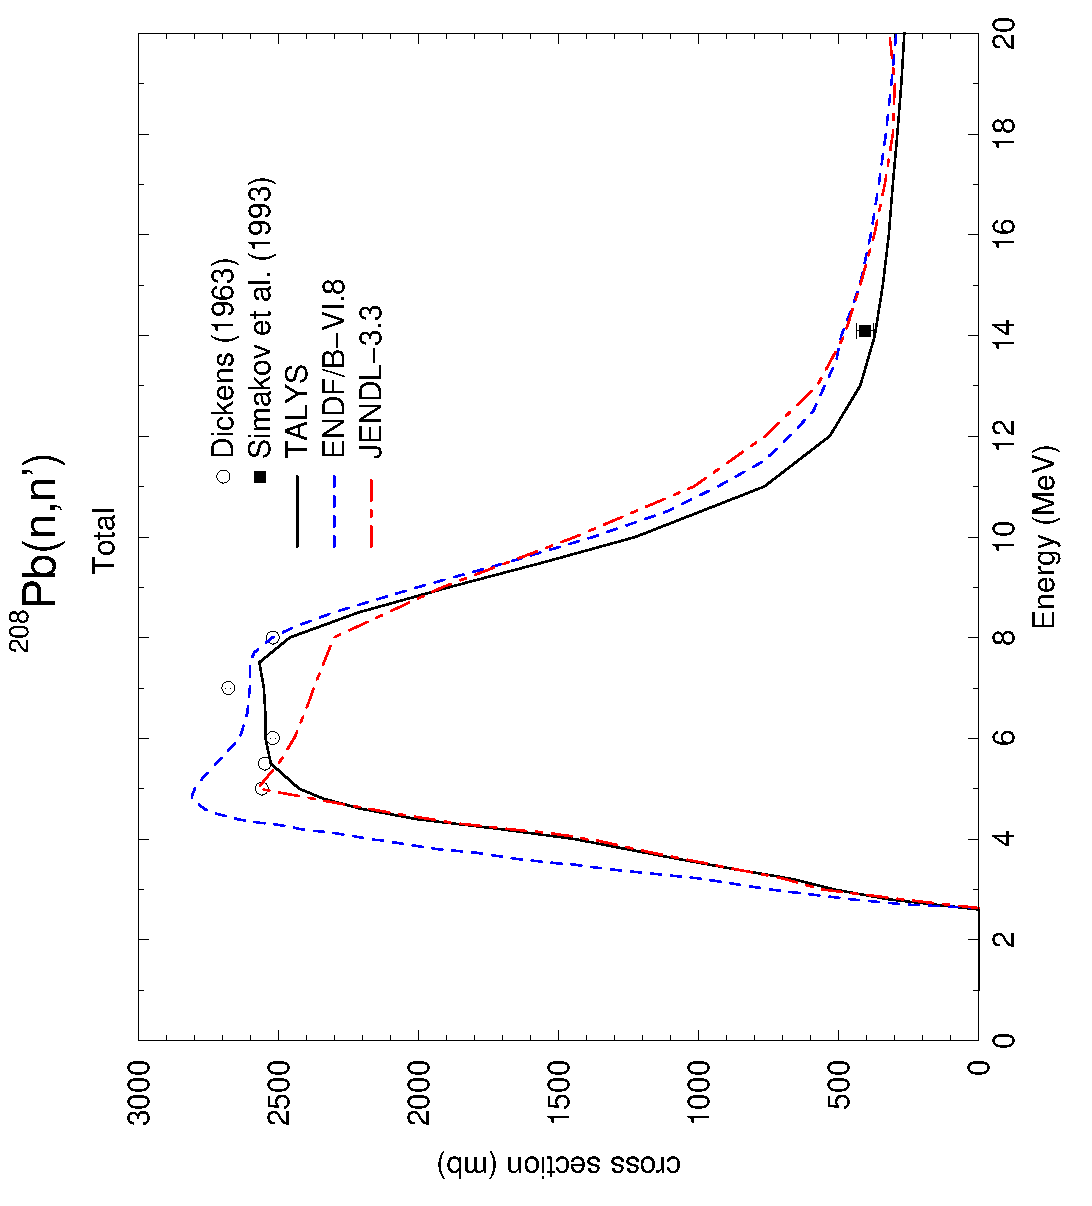
\includegraphics[scale=0.5,angle=270]{MT4} \centering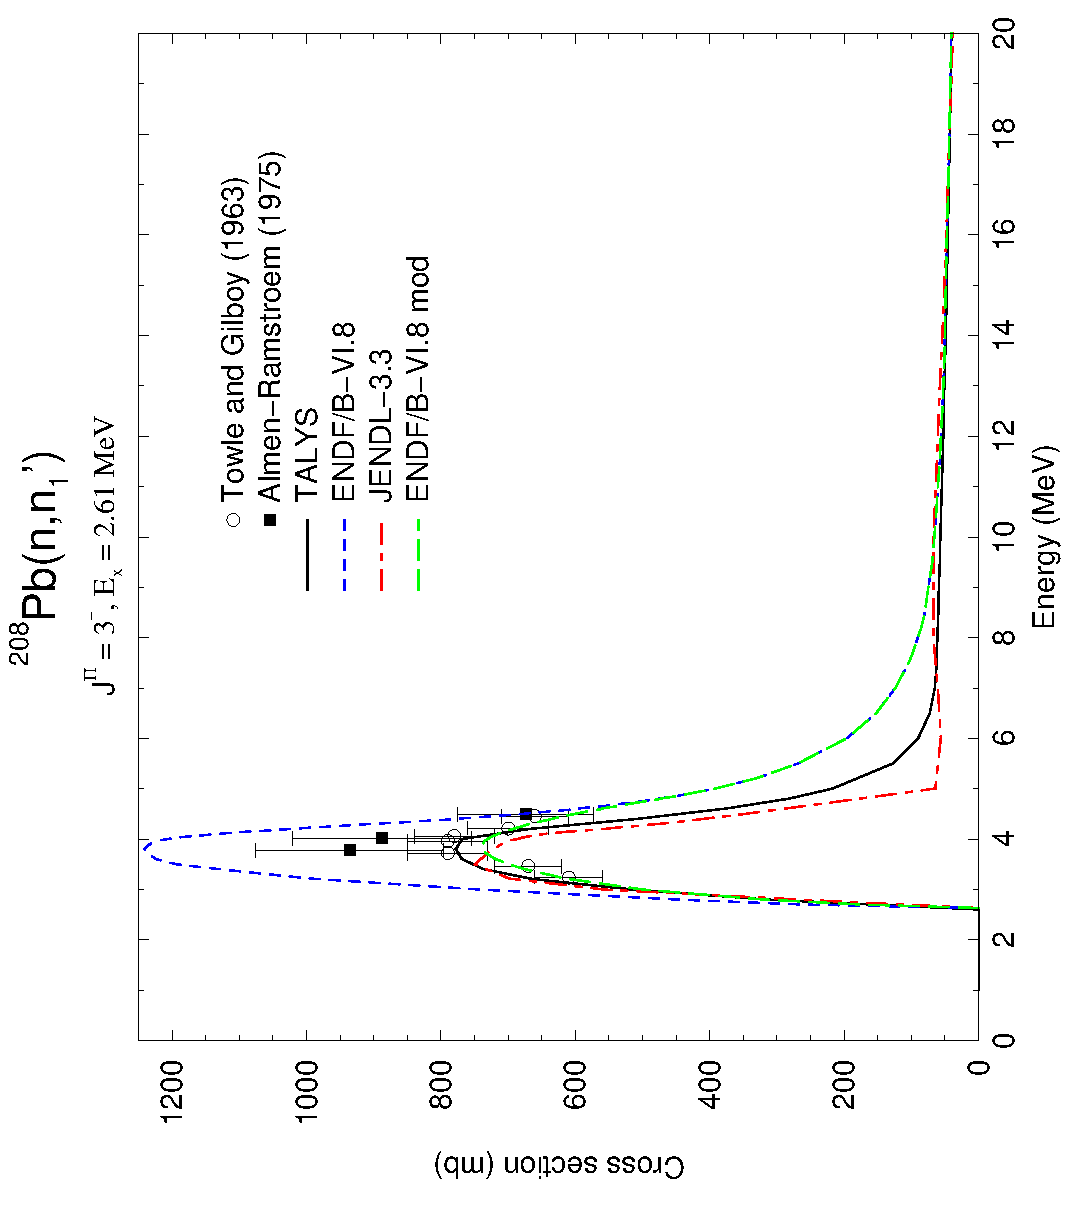
\includegraphics[scale=0.5,angle=270]{MT51}
}
\centerline{
\centering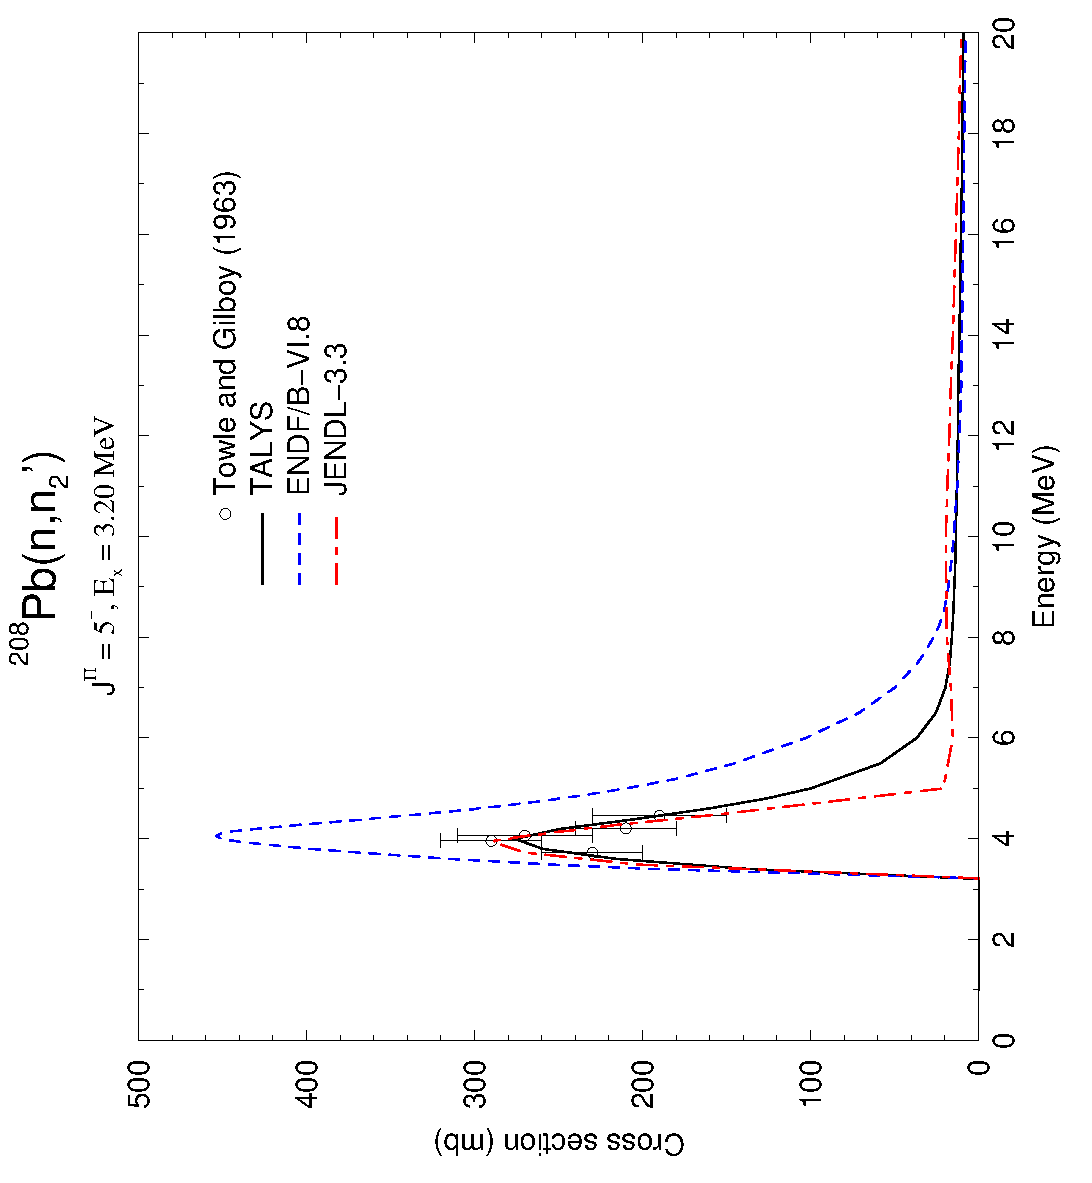
\includegraphics[scale=0.5,angle=270]{MT52} \centering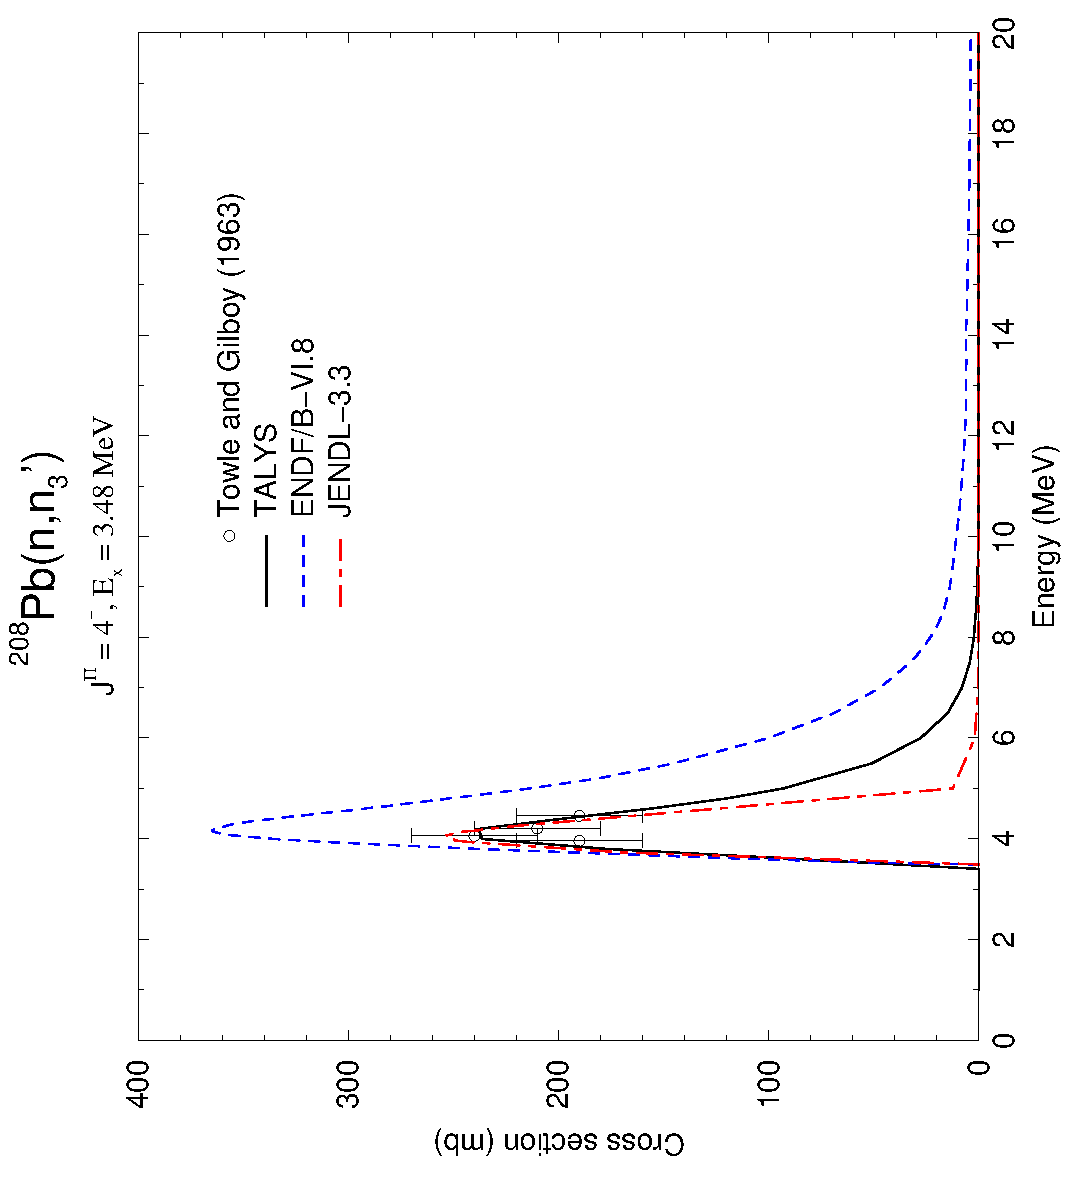
\includegraphics[scale=0.5,angle=270]{MT53}
}
\caption{Partial cross sections for neutrons incident on ${}^{208}$Pb.}
\label{pbpart1}
\end{figure}
\begin{figure}
\vspace*{-15mm}
\centerline{
\centering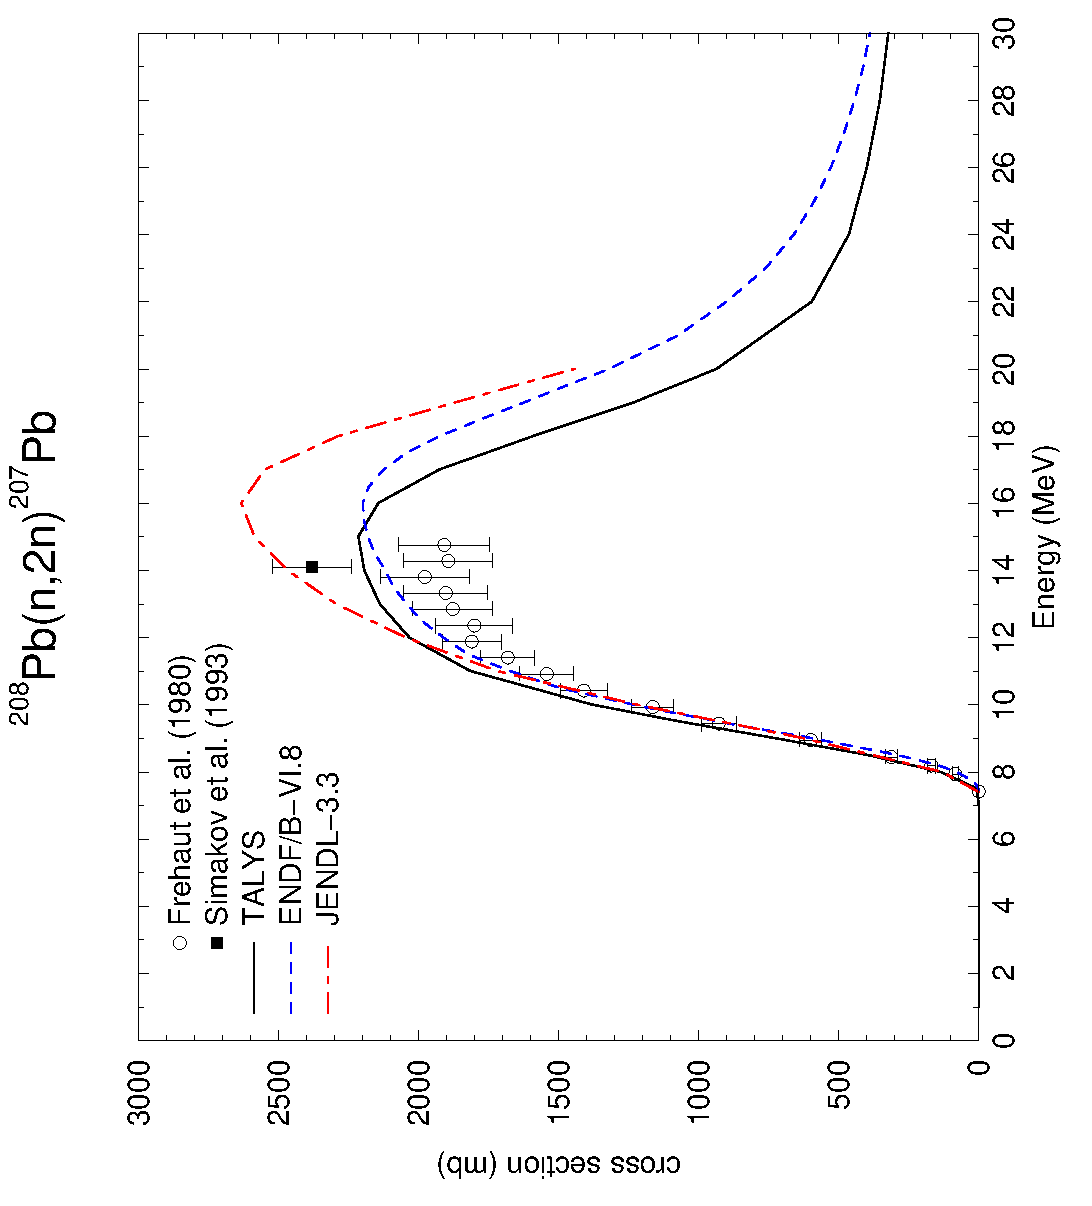
\includegraphics[scale=0.5,angle=270]{MT16} \centering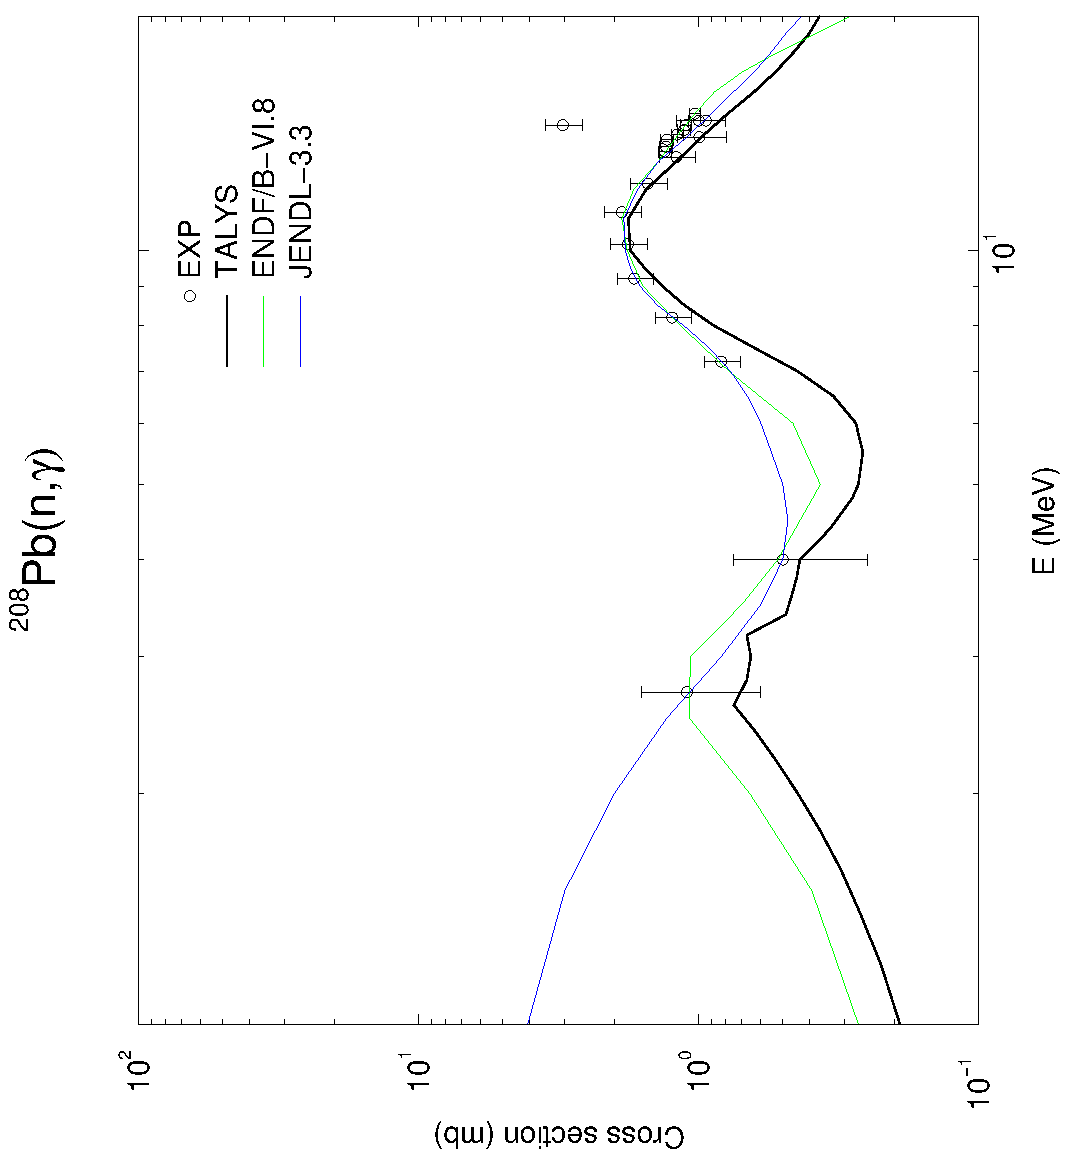
\includegraphics[scale=0.5,angle=270]{MT102}
}
\centerline{
\centering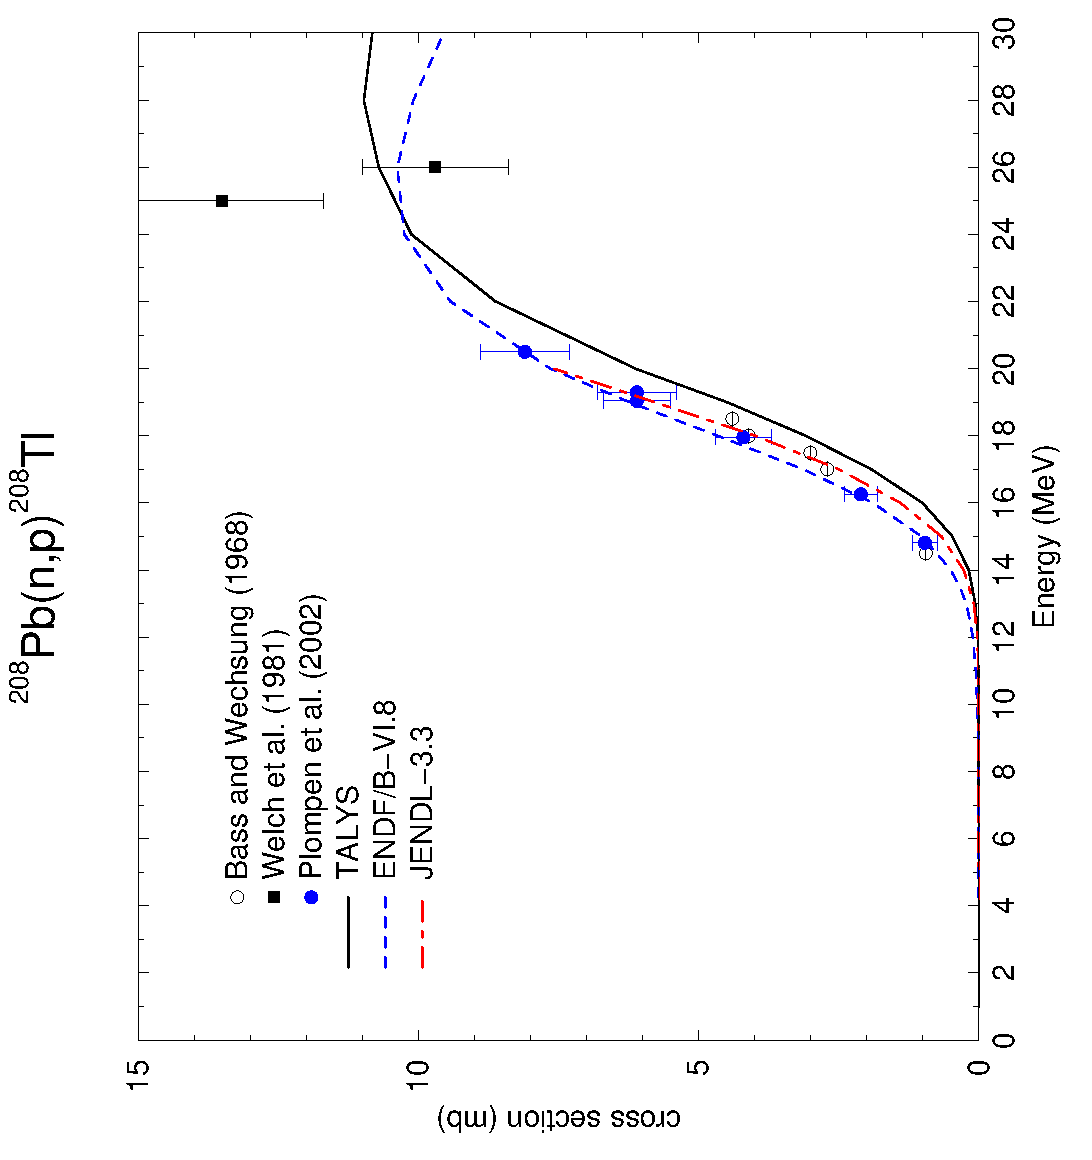
\includegraphics[scale=0.5,angle=270]{MT103} \centering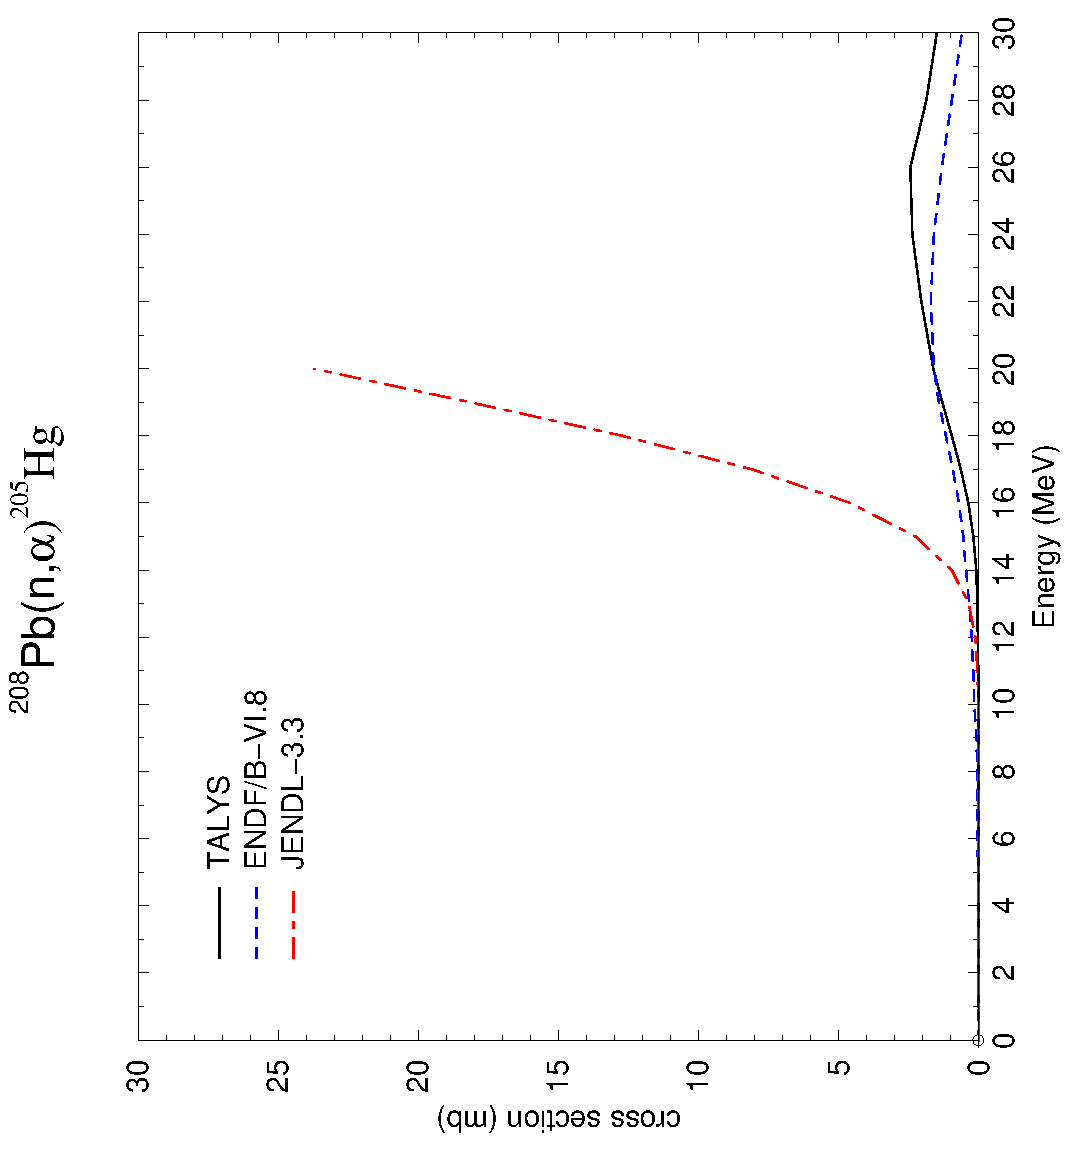
\includegraphics[scale=0.5,angle=270]{MT107}
}
\caption{Partial cross sections for neutrons incident on ${}^{208}$Pb.}
\label{pbpart2}
\end{figure}
